\documentclass[12pt]{article}

\usepackage{listings}
\usepackage{array}
\usepackage{inconsolata}
\usepackage{color}
\usepackage{matlab-prettifier}
\usepackage{amsmath}
\usepackage[utf8]{inputenc}
\usepackage[T1]{fontenc}
\usepackage{lmodern}
\usepackage{minted}
\usepackage{graphicx}
\usepackage{tabularx}
\usepackage{tikz}
\usetikzlibrary{shapes,arrows,arrows.meta, positioning, calc, shapes.geometric, shadows}
\graphicspath{{assets/}}

\usepackage{hyperref}
\hypersetup{
    colorlinks,
    citecolor=black,
    filecolor=black,
    linkcolor=black,
    urlcolor=black
}

\newcommand{\fullwidthimage}[1]{
    \begin{center}
        \makebox[\textwidth]{\includegraphics[width=\paperwidth]{#1}}
    \end{center}
}

\newcommand{\customwidthimage}[2]{
    \begin{center}
        \makebox[\textwidth]{\includegraphics[width=#2]{#1}}
    \end{center}
}

\newminted{matlab}{frame=lines, framesep=2mm, baselinestretch=1.2, fontsize=\footnotesize, linenos, style=friendly, breaklines}
\renewcommand\contentsname{Tartalomjegyzék}

\begin{document}

\title{Szenzormodalitások}
\author{Jegyzet}
\date{}
\maketitle

\clearpage

\tableofcontents

\clearpage

\section{Vizsga kérdések}

\subsection{Szenzorok}
\subsubsection{Szenzor definíció}
\begin{itemize}
    \item A szenzor egy eszköz, ami fizikai ingereket (pl.: hőmérséklet, fény, nyomás) érzékel és ezeket mérhető jelekké alakítja.
    \item Ezek a jelek lehetővé teszik környezetünk változásainak észlelését és mérését. (pl.: ipar, egészségügy, környezetvédelem)
    \item Szenzorok lehetnek aktív vagy passzív típusúak, azaz saját energiát használó vagy a környezeti energiát felhasználó eszközök.
    \item Digitális adatot ad ki magából.
    \item A digitális adatot tovább adja küldeni vezetékes vagy vezeték nélküli csatornán.
\end{itemize}

\subsubsection{Szenzor kategóriák}
\begin{itemize}
    \item Hőmérséklet-szenzorok
    \begin{itemize}
        \item Környezet hőmérsékletének mérése, gyakran használják otthoni fűtési rendszerekben, autókban és ipari folyamatokban.
    \end{itemize}
    \item Gyorsulásmérők
    \begin{itemize}
        \item Gyorsulás/rezgés mértékét érzékelik, gyakran használják mobiltelefonok képernyő-orientációjának szabályozásához, járművek ütközésérzékelésére, épületek szeizmikus monitorozására.
    \end{itemize}
    \item Kémiai szenzorok
    \begin{itemize}
        \item Vegyületek mérése levegőben, vízben vagy egyéb közegben.
        \item Környezetszennyezés monitorozása, ipari folyamatok ellenőrzése, egészségügyben.
    \end{itemize}
    \item Hangfrekvencia-szenzorok
    \begin{itemize}
        \item Hanghullámokat érzékel, alkalmazhatóak biztonsági rendszerekben, hangfelismerésben és akusztikai elemzésben.
    \end{itemize}
\end{itemize}

\subsubsection{Szenzorok használati területei}
\begin{quote}
    A szenzorok javítják életünk minőségét, hatékonyságát és biztonságát.
\end{quote}
\begin{itemize}
    \item Okostelefonok és viselhető eszközök
    \begin{itemize}
        \item Gyorsulásmérők, giroszkópok, lépésszámlálás, automatikus fényerő-szabályozás.
    \end{itemize}
    \item Otthoni automatizálás és intelligens otthonok
    \begin{itemize}
        \item Hőmérséklet, fény, mozgás
    \end{itemize}
    \item Ipari automatizálás
    \begin{itemize}
        \item Üzemeltetés hatékonyságát növeli.
    \end{itemize}
    \item Egészségügy és orvostechnika
    \begin{itemize}
        \item Kémiai szenzorok, biometrikus szenzorok, diagnosztikák/kezelések monitorozása
    \end{itemize}
    \item Autóipar
    \begin{itemize}
        \item Ütközésérzékelők, parkolássegítő rendszerek
    \end{itemize}
    \item Biztonsági rendszerek
    \begin{itemize}
        \item Mozgásérzékelők, füstérzékelők, kamera szenzorok a veszélyhelyzetek azonosítására.
    \end{itemize}
\end{itemize}

\clearpage
\subsubsection{Szenzor problémák}
\begin{itemize}
    \item Kalibrációs problémák
    \begin{itemize}
        \item Következménye a pontatlanság lehet, kell a rendszeres kalibráció a pontos működéshez.
    \end{itemize}
    \item Környezeti hatások
    \begin{itemize}
        \item Extrém hőmérsékletek, por és egyéb környezeti tényezők befolyásolhatják a szenzorok teljesítményét.
    \end{itemize}
    \item Energiafogyasztás
    \begin{itemize}
        \item Akkumulátorral működő eszközöknél a szenzorok sokat fogyasztanak.
    \end{itemize}
    \item Inferencia és zaj
    \begin{itemize}
        \item Zajok torzíthatják a szenzorok által gyűjtött adatokat, ami pontatlansághoz vezet.
    \end{itemize}
    \item Technológiai korlátok (Például kommunikáció)
\end{itemize}

\subsubsection{Aktuátor definíció, példák}
\begin{quote}
    Az aktuátorok olyan eszközök, amik elektromos jelet fizikai műveletekké alakítanak át, az aktuátorok lehetnek mechanikus szerkezetek vagy bonyolultabb rendszerek.
\end{quote}
\begin{itemize}
    \item Elektromos motorok
    \begin{itemize}
        \item Elektromos energiát mechanikai mozgássá alakítanak át, járművek meghajtását teszik lehetővé például.
    \end{itemize}
    \item Hidraulikus aktuátorok
    \begin{itemize}
        \item Folyadék nyomásának növelésével/csökkentésével működnek, erős és precíz mozgatásra képesek, például építőipari gépekben.
    \end{itemize}
    \item Pneumatikus aktuátorok
    \begin{itemize}
        \item Sűrített levegőt használnak a mozgás előidézésére, például ahol gyors és ismétlődő mozgásra van szükség.
    \end{itemize}
\end{itemize}

\subsection{DAQ/Tradícionális vezérlés/DCS/SCADA/Monitoring/Vezérlőrendszerek}
\subsubsection{DIKW piramis}
\begin{quote}
    Tudáspiramis, egy modell, bemutatja hogyan alakulnak át az adatok értelmezhető és használható tudássá.
\end{quote}
\begin{enumerate}
    \item Adat (Nyers adatok kontextus nélkül (pl.: mérések adatai), kevés hasznos információt tartalmaznak.)
    \item Információ (Adatok kontextusba helyezése.)
    \item Tudás (Információkból következtetéseket lehet levonni.)
    \item Bölcsesség (Tudás alkalmazása, miértje.)
\end{enumerate}

\subsubsection{Tradícionális vezérlési rendszerek vs. Elosztott vezérlési rendszerek (DCS)}
\begin{itemize}
    \item Tradícionális vezérlési rendszerek
    \begin{itemize}
        \item Központosított architektúrára épül, ahol egy vagy több központi vezérlőegység végzi a folyamatok összes vezérlési és felügyeleti feladatát.
        \item Egyszerű, alacsony költségek
        \item Korlátozott skálázhatóság, a központosított vezérlés miatt nagyobb a rendszer kiesésének kockázata
    \end{itemize}
    \item Elosztott vezérlési rendszerek (DCS)
    \begin{itemize}
        \item Vezérlési folyamatokat moduláris egységek között osztja szét, amik kommunikálnak egymással egy közös hálózaton keresztül.
        \item Minden egyes szegmens a saját területéért felelős.
        \item Magasabb rendelkezésre állás, megbízhatóság, skálázhatóság
        \item Költséges, bonyolult
    \end{itemize}
\end{itemize}

\subsubsection{DAQ rendszer előnyök/hátrányok, alkalmazási területek}
\begin{quote}
    Adatgyűjtő rendszerek, lehetővé teszik fizikai jelenségek valós idejű monitorozását és analízisét. \\
    Egy tipikus DAQ rendszer szenzorokból áll, adatgyűjtő hardverből és szoftverből áll, amik összegyűjtik és feldolgozzák az adatokat.
\end{quote}
\begin{itemize}
    \item Előnyök (Rugalmas konfiguráció, pontos mérések, valós idejű adatfeldolgozás, automatizálás)
    \item Hátrányok (Költségek, technikai komplexitás, hardver és szoftverkompatibilitás, Karbantartás, frissítések)
    \item Alkalmazási területek (Tudományos kutatás, mérnöki tesztelés és fejlesztés, környezeti monitorozás, egészségügy)
\end{itemize}

\subsubsection{Elosztott vezérlési rendszerek (DCS)}
\begin{itemize}
    \item Előnyök (Magasabb rendelkezésre állás, megbízhatóság, skálázhatóság)
    \item Hátrányok (Költséges, bonyolult)
    \item Alkalmazási területek (Gyógyszeripar, erőművek, élelmiszeripar)
\end{itemize}

\subsubsection{SCADA rendszer}
\begin{itemize}
    \item Előnyök (Távoli felügyelet, valós idejű adatgyűjtés, megbízhatóság, automatizálás)
    \item Hátrányok (Komplexitás, költségek, karbantartás)
    \item Alkalmazási területek (Energiaipar, közlekedés, gyártás és automatizálás)
\end{itemize}

\clearpage
\subsection{DAQ}
\subsubsection{DAQ rendszer komponensei}
\begin{itemize}
    \item Szenzorok és érzékelők (Fizikai változások elektromos jelekké alakítja át)
    \item Jelkondicionáló áramkörök (Jeleket átalakítja, hogy azok megfelelőek legyenek)
    \item Adatgyűjtő eszközök - DAQ hardver (Előkészített analóg jeleket digitális formátumba konvertálja)
    \item Számítógép és interfész (DAQ hardvert számítógéphez kell csatlakoztatni, interfész lehet USB, PCI, PCIe, Ethernet és szoftveren keresztül kezeli az adatokat)
    \item Szoftver (LabVIEW, MATLAB)
\end{itemize}

\subsubsection{DAQ alkalmazási területek}
\begin{itemize}
    \item Tudományos kutatás, mérnöki tesztelés és fejlesztés, környezeti monitorozás, egészségügy
\end{itemize}

\subsubsection{Jelkondícionálás}
\begin{quote}
    A jelkondícionálás előkészíti az elektromos jeleket a digitális átalakításra és feldolgozásra, célja, hogy javítsa a jelek minőségét és növelje az adatgyűjtés pontosságát.
\end{quote}
\begin{itemize}
    \item Erősítés, szűrés, hőmérséklet-kompenzáció, lineárizáció, galvanikus leválasztás, jelalakítás
\end{itemize}

\subsubsection{Betegmonitorozó DAQ infrastruktúra}
\begin{quote}
    Beteg valós időben történő monitorozása.
\end{quote}
\begin{itemize}
    \item Szenzorok és érzékelők, jelkondícionáló áramkörök, adatgyűjtő eszközök, központi monitorozó állomás és hálózati infrastruktúra, szoftver és analitikai eszközök, adattárolás és archiválás
\end{itemize}

\subsubsection{DAQ rendszerek kihívásai}
\quote
\begin{itemize}
    \item Jelzaj és interferencia, nagy adatmennyiség kezelése, szenzor kalibráció és hőmérsékleti hatások, Adatbiztonság és adatvédelem, hardver és szoftverkompatibilitás, skálázhatóság és rugalmasság, Kezelhetőség 
\end{itemize}

\subsection{Elosztott vezérlési rendszerek (DCS)}
\subsubsection{DCS architektúra}
\begin{itemize}
    \item Vezérlési folyamatokat moduláris egységek között osztja szét, amik kommunikálnak egymással egy közös hálózaton keresztül.
    \item Minden egyes szegmens a saját területéért felelős.
    \item Moduláris
\end{itemize}

\subsubsection{DCS komponensei}
\begin{itemize}
    \item Folyamatvezérlők
    \item Operátori állomások (HMI)
    \item I/O modulok
    \item Kommunikációs hálózatok
    \item Mérnöki munkaállomások
    \item Adatarchiváló és elemző rendszer
    \item Biztonsági rendszerek
\end{itemize}

\subsubsection{DCS előnyök és hátrányok}
\begin{itemize}
    \item Előnyök (Magasabb rendelkezésre állás, megbízhatóság, skálázhatóság)
    \item Hátrányok (Költséges, bonyolult)
\end{itemize}

\subsubsection{DCS alkalmazási területek}
\begin{itemize}
    \item Gyógyszeripar, erőművek, élelmiszeripar
\end{itemize}

\subsection{Supervisory control and data acquisition - SCADA}
\subsubsection{SCADA architektúra, komponensei}
\begin{quote}
    Lehetővé teszik a nagy ipari és infrastrukturális folyamatok távoli monitorozását, vezérlését és automatizálását.
\end{quote}
\begin{itemize}
    \item Terepi eszközök
    \item Távközlési rendszerek
    \item RTU-k
    \item SCADA szerverek és számítógépek
    \item HMI
    \item Adatbázis és archiváló rendszerek
    \item Biztonsági komponensek
    \item Alkalmazási és szoftvereszközök
\end{itemize}

\subsubsection{SCADA előnyök/hátrányok}
\begin{itemize}
    \item Előnyök (Távoli felügyelet, valós idejű adatgyűjtés, megbízhatóság, automatizálás)
    \item Hátrányok (Komplexitás, költségek, karbantartás)
\end{itemize}

\subsubsection{SCADA alkalmazási területek}
\begin{itemize}
    \item Energiaipar, közlekedés, gyártás és automatizálás
\end{itemize}

\clearpage
\subsubsection{SCADA funkciói}
\begin{itemize}
    \item Távmérések, távjelzések fogadása
    \item Visszajelzés, adat vizualizáció
    \item Naplózás
    \item Riasztások (határérték és gradiens figyelés)
    \item Topológia analízis
    \item Távparancsadás
    \item Autentikáció és jogosultságkezelés
    \item Adattárolás
\end{itemize}

\subsubsection{Basic SCADA vs. Integrated SCADA vs. Networked SCADA}
\begin{itemize}
    \item Basic SCADA
    \begin{itemize}
        \item Alapvető távoli felügyelet és adatgyűjtés
        \item Korlátozott I/O kapacitás, egyszerű HMI és adatgyűjtés
        \item Kis teljesítményűek, egyszerű ipari folyamatok
    \end{itemize}
    \item Integrated SCADA
    \begin{itemize}
        \item Bonyolultabb, több funkciót integrálnak egyetlen koherens rendszerben.
        \item ERP rendszerek, komplex gyártási folyamatok, nagy létesítmények, vállalati szintű
    \end{itemize}
    \item Networked SCADA
    \begin{itemize}
        \item Széleskörű hálózati kapcsolatok, távoli elérés és vezérlés, adatmegosztás a létesítmények között, felhőalapú adattárolás és szolgáltatások
        \item Távvezetéki rendszerek, vízellátás, energiaelosztás, szétszórt infrastruktúra felügyelet
    \end{itemize}
\end{itemize}

\clearpage
\subsection{Biojel-gyűjtés (Biosignal acquisition)}
\begin{quote}
    A bioszignálok az élőlények testéből származó elektromos, mechanikai vagy más fizikai jelek, amik információt hordoznak az adott szervezet vagy szervrendszer állapotáról.
\end{quote}

\begin{itemize}
    \item Elektromos bioszignálok (Ideg és izomsejtek elektromos aktivitásából származnak)
    \begin{itemize}
        \item \textbf{EKG} (Elektrokardiogram), szív elektromos tevékenysége.
        \item \textbf{EEG} (Elektroenkefalográfia), Agy elektromos aktivitása.
        \item \textbf{EMG} (Elektromiográfia), izom elektromos aktivitása.
    \end{itemize}
    \item Mechanikai bioszignálok (Fizikai mozgások és változások)
    \begin{itemize}
        \item \textbf{Pulzushullám-velocitás}, az artériás rugalmasság mérésére szolgáló jel.
        \item \textbf{Spirometria}, légzés mechanikájának mérése.
    \end{itemize}
    \item Kémiai és biokémiai bioszignálok (Kémiai összetétel változásai)
    \begin{itemize}
        \item \textbf{Glükózszint-mérés}, vércukorszint mérés.
        \item \textbf{pH-mérés}, testfolyadék savasságának mérése.
    \end{itemize}
    \item Optikai és termikus bioszignálok (Fény és hő alapú jelek)
    \begin{itemize}
        \item \textbf{Pulzoximetria}, véroxigénszint mérés.
        \item \textbf{Testhőmérséklet-mérés}, a test belső hőmérsékletének mérési módjai.
    \end{itemize}
    \item Környezeti tényezők és egyéb mérések
    \begin{itemize}
        \item \textbf{Páratartalom és hőmérséklet}
        \item \textbf{Tartás és gyorsulás}
    \end{itemize}
\end{itemize}

\subsubsection{Szenzoradat kezelési folyamat}
\begin{enumerate}
    \item Data acquisition (DAQ) (egy/több szenzor)
    \item Adatkezelés (feldolgozás/szűrés)
    \item Tárolás, keresés
    \item Vizualizáció
    \item Megosztás
\end{enumerate}

\subsubsection{Mérési hibák (típusok/források)}
\begin{quote}
    Minden mérés tartalmaz hibákat!
\end{quote}
\begin{itemize}
    \item Rendszerszerű hibák
    \begin{itemize}
        \item \textbf{Kalibrációs hibák} (Mérőeszközök nem megfelelő kalibrálása)
        \item \textbf{Elektromos interferencia} (Környezeti elektromos berendezések zavarai)
        \item \textbf{Jelátviteli hiba} (Hosszú vagy rossz minőségű kábelezés)
    \end{itemize}
    \item Random hibák
    \begin{itemize}
        \item \textbf{Operátori hiba} (Emberi tényező, mint pl.: szenzor helytelen elhelyezése)
        \item \textbf{Fiziológiai zaj} (A testből származó nem kívánt jelek, pl.: izomzaj)
        \item \textbf{Mintavételi hiba} (Nem megfelelő mintavételi frekvencia alkalmazása)
    \end{itemize}
\end{itemize}

\clearpage
\subsubsection{Egyetlen vs. több szenzoros mérési problémák}
\begin{itemize}
    \item Egyetlen szenzoros mérési problémák
    \begin{itemize}
        \item \textbf{Korlátozott információszerzés}, egyetlen nézőpontból származó adatok korlátozott betekintést nyújtanak.
        \item \textbf{Hibatűrés hiánya}, egy szenzor meghibásodásánál nincs redundancia, ami az egész mérési folyamat kieséséhez vezethet.
        \item \textbf{Nagyobb kockázat a pontatlanságokra}, az adatok értelmezésekor
    \end{itemize}
    \item Több szenzoros mérési problémák
    \begin{itemize}
        \item \textbf{Adatkezelés és feldolgozás}, nagy adatmennyiség kezelése, tárolása, elemzése bonyolult, időigényes
        \item \textbf{Adatfúzió és integráció}, a különböző típusú és forrású adatok összeegyeztetése és integrálása technikai kihívást jelenthet.
        \item \textbf{Interferencia és koherencia}, a szenzorok közötti interferencia és az adatok koherenciájának hiánya torzíthatja az eredményeket.
    \end{itemize}
\end{itemize}

\clearpage
\subsubsection{Mérnöki kihívások a nagymennyiségű adatgyűjtésnél}
\begin{itemize}
    \item Általános kihívások
    \begin{itemize}
        \item P1 $\rightarrow$ Sok DAQ csomópont
        \item P2 $\rightarrow$ Sok szenzor (különböző típusú)
        \item P3 $\rightarrow$ Nagy adatmennyiség lehetőleg gyorsan átküldve
    \end{itemize}
    \item Kommunikációs probléma $\rightarrow$ P1 $\times$ P2 $\times$ P3
    \item Szoftver kihívások
    \begin{itemize}
        \item Valós idejű DAQ + előfeldolgozás + feldolgozás + megjelenítés (különböző tartományok)
        \item Komplex döntési helyzetek
        \item Online adatmenedzsment (megosztás + archiválás)
    \end{itemize}
    \item Hardver korlátok
    \begin{itemize}
        \item Energia problémák
        \item Kommunikációs hatótávolságok, adat multiplexálási problémák/idő, frekvencia
        \item Biztonság, megbízhatóság, használhatóság
    \end{itemize}
\end{itemize}
\section{Téma 1}

\subsection{Szenzor/érzékelő}
\begin{itemize}
    \item Monitorozásnál a szenzor
    \begin{itemize}
        \item Érzékelő ami valamilyen fizikai/kémiai mennyiséget, vagy annak változását méri.
        \item Digitális adatot ad ki magából.
        \item A digitális adatot tovább tudja küldeni \textbf{vezetékes}, vagy \textbf{vezeték nélküli} csatornán.
    \end{itemize}
    \item Szenzor problémák
    \begin{itemize}
        \item Elem
        \item Kezelhetőség
        \item Működési időtartam
        \item Élettartam
        \item Kábelek, környezeti beépítési problémák
        \item Egészségkárosító hatás
        \item Technológiai korlátok (kommunikációs hatótávolság)
    \end{itemize}
\end{itemize}

\subsection{Adat-Információ-Ismeret-Tudás piramis}
\begin{center}
    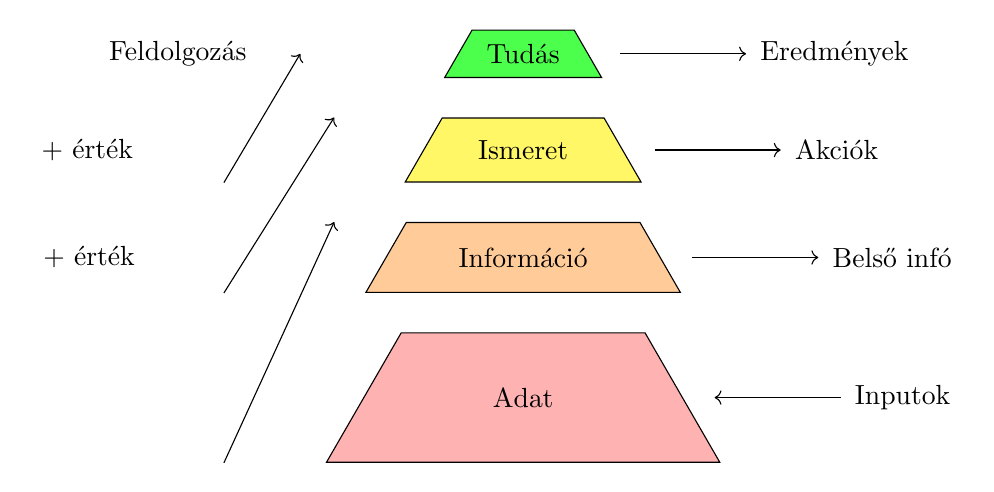
\begin{tikzpicture}[every node/.style={draw, anchor=south, inner sep=5pt}]
        % Define nodes
        \node[trapezium, trapezium angle=60, minimum width=5cm, fill=red!30] (data) {Adat};
        \node[trapezium, trapezium angle=60, minimum width=4cm, fill=orange!40, above=0.5cm of data] (info) {Információ};
        \node[trapezium, trapezium angle=60, minimum width=3cm, fill=yellow!60, above=0.5cm of info] (knowledge) {Ismeret};
        \node[trapezium, trapezium angle=60, minimum width=2cm, fill=green!70, above=0.5cm of knowledge] (wisdom) {Tudás};
    
        % Define labels on the right side
        \node[anchor=west, draw=none, fill=none] (dataLabel) at ([xshift=2cm]data.east) {Inputok};
        \node[anchor=west, draw=none, fill=none] (infoLabel) at ([xshift=2cm]info.east) {Belső infó};
        \node[anchor=west, draw=none, fill=none] (knowledgeLabel) at ([xshift=2cm]knowledge.east) {Akciók};
        \node[anchor=west, draw=none, fill=none] (wisdomLabel) at ([xshift=2cm]wisdom.east) {Eredmények};
    
        % Draw arrows with some space between the trapeziums and the arrows on the right
        \draw[->] (dataLabel.west) -- ([xshift=0.4cm]data.east);
        \draw[<-] (infoLabel.west) -- ([xshift=0.4cm]info.east);
        \draw[<-] (knowledgeLabel.west) -- ([xshift=0.4cm]knowledge.east);
        \draw[<-] (wisdomLabel.west) -- ([xshift=0.4cm]wisdom.east);
    
        % Define labels on the left side
        \node[anchor=east, draw=none, fill=none] at ([xshift=-3cm]info.west) (dataValue) {+ érték};
        \node[anchor=east, draw=none, fill=none] at ([xshift=-3.5cm]knowledge.west) (infoValue) {+ érték};
    
        % Place "Feldolgozás" at the top arrow
        \node[anchor=east, draw=none, fill=none] at ([xshift=-2.5cm]wisdom.west) (process) {Feldolgozás};
    
        % Draw arrows vertically between the levels on the left side
        \draw[->] ([xshift=-3.8cm]data.south) -- ([xshift=-2.4cm]info.north);
        \draw[->] ([xshift=-3.8cm]info.south) -- ([xshift=-2.4cm]knowledge.north);
        \draw[->] ([xshift=-3.8cm]knowledge.south) -- ([xshift=0.5cm]process.east);
    
    \end{tikzpicture}
\end{center}

\subsection{Data Acquisition - DAQ rendszerek}
\begin{itemize}
    \item Szenzorok
    \item Kliens oldali adatgyűjtő eszközök
    \begin{itemize}
        \item Megjelenítési felülettel, vagy anélkül
        \item Általános célú megoldások (PC, mini PC, okos telefon)
        \item Célhardverek
    \end{itemize}
    \item Központi adat tároló és adat menedzselő rendszerek (adat szerverek)
    \item Központi/kliens oldali megjelenítő rendszerek (web/alkalmazás szerverek)
    \item Központi rendszer felügyeleti eszközök (alkalmazás szerverek)
    \item Üzemeltető és kiszolgáló személyzet infrastruktúrája (szakemberek, technikusok, CallCenter, stb.)
    \item Kommunikációs infrastruktúra, ami az egyes részeket összeköti.
\end{itemize}

\subsection{Járulékos hardver eszközök}
\begin{itemize}
    \item Összeköttetéshez a központi irányába
    \begin{itemize}
        \item Okostelefon
        \item Számítógép/célszámítógép/PDA
    \end{itemize}
    \item Kábelek a szenzor és az adatgyűjtő összeköttetéshez
    \item Dongle-ek a vezetéknélküli átvitelhez
\end{itemize}

\subsection{Rendszerirányító rendszerek}
\begin{itemize}
    \item Valós idejű információ folyamatos továbbítása, tárolása és feldolgozása, a rendszerirányítás megbízható számítógépes támogatása mind az operatív üzemirányítás, mind az üzemelőkészítés és üzemértékelés elvégzéséhez.
    \item Központi vezérlési rendszerek
    \item Distributed Control System - DCS
    \item Supervisory control and data acquisition - SCADA
\end{itemize}

\subsubsection{Distributed Control System - DCS}
\begin{itemize}
    \item Szemben a direkt helyi vezérlővel megvalósított rendszerekkel:
    \begin{itemize}
        \item a DCS-ek esetében nagyobb a megbízhatóság,
        \item kisebbek a kialakítási költségek, mivel a vezérlés lokálisan megvalósított és a vezérléshez szükséges kommunikáció is lokális,
        \item központi (akár távolról megvalósított) ellenőrzés
    \end{itemize}
\end{itemize}

\subsubsection{Supervisory Control and Data Acquisition - SCADA}
\begin{itemize}
    \item Felügyeleti szabályozás és adatgyűjtés
    \begin{itemize}
        \item Központosított vezérlés (figyel és vezérel)
        \item Távoli adatgyűjtől
        \item Biztonságos kommunikáció
        \item Elosztott adattárolás
        \item Időbélyegek
        \item Például $\rightarrow$ Erőművek, csővezetékek, elektromos hálózatok, vízhálózatok
    \end{itemize}
    \item \underline{\textbf{S}}upervisory $\rightarrow$ Operator, engineer, supervisor
    \item \underline{\textbf{C}}ontrol $\rightarrow$ Monitoring, Limited, Telemetry, Remote/Local
    \item \underline{\textbf{D}}ata \underline{\textbf{A}}cquisition $\rightarrow$ Analog/Digital
\end{itemize}

\customwidthimage{scada}{8cm}

\subsubsection{SCADA rendszer generációk}
\begin{itemize}
    \item Monolitikus, szigetszerű rendszerek, egymástól függetlenül működő zárt (kapcsolat nélküli)
    \item Elosztott rendszerek $\rightarrow$ LAN hálózatba rendezett, egymással hálózati protokollokon kommunikáló
    \item Hálózatos rendszerek $\rightarrow$ Földrajzilag nagyobb kiterjedésű (LAN-nál nagyobb) hálózatokba rendezett, egymással hálózati protokollokon kommunikáló rendszerek, egymástól független, egymással párhuzamosan futó
    \item Internet of Things (IoT)
    \item Felhő infrastruktúrákkal támogatott, növelt hatékonysággal, és optimált költségekkel üzemelő online, valós idejű rendszerek.
\end{itemize}

\subsubsection{SCADA rendszer általános belső architektúrája}
\customwidthimage{scada_arch}{15cm}

\clearpage
\subsubsection{A SCADA rendszerek főbb funkciói}
\begin{itemize}
    \item Távmérések, távjelzések fogadása
    \item Visszajelzés, adat vizualizáció
    \item Naplózás
    \item Riasztások (határérték és gradiens figyelés)
    \item Topológia analízis
    \item Távparancsadás
    \item Autentikáció és jogosultságkezelés
    \item Adattárolás
\end{itemize}

\subsection{Példák a távoli adatgyűjtésre}
\begin{quote}
    Régebben távoli, nehezen megközelíthető, veszélyes helyeken mérés, illetve gyakori automatizált méréssorozatok esetén elterjedt.
\end{quote}
\begin{itemize}
    \item Mérő állomásoknál
    \begin{itemize}
        \item Meterológiai, vízállás mérő állomások, épületek/hidak/alagutak
    \end{itemize}
    \item Komplex berendezések
    \begin{itemize}
        \item Részecskegyorsítók
    \end{itemize}
    \item Egészséges emberek monitorozása
    \begin{itemize}
        \item Intelligens ruhák
        \item Munka közben (katonaság, tűzoltóság)
        \item Sportolás közben (fitness)
    \end{itemize}
    \item Telemedicina
    \begin{itemize}
        \item Távdiagnózis
        \item Távmonitorozás
    \end{itemize}
    \item Autonóm robotok
    \begin{itemize}
        \item AUV, UAV, ROV
    \end{itemize}
\end{itemize}

\subsubsection{Távoló adatgyűjtő rendszerek általános működése}
\begin{itemize}
    \item Érzékelés
    \item Adattovábbítás
    \item Adatfeldolgozás, adatszűrés
    \item Adatelemzés
    \item Adatmegosztás, vizualizáció
    \item Az adatgyűjtő rendszer üzemeltetése
    \begin{itemize}
        \item Megjelenő hibák észlelése és korrigálása
    \end{itemize}
\end{itemize}

\subsection{Általános páciens monitorozó DAQ architektúra}
\customwidthimage{altpac}{15cm}

\subsection{Élettani paraméterek monitorozása extrém körülmények között}
\begin{center}
    \customwidthimage{eletext}{14cm}
    \customwidthimage{eletext2}{14cm}
\end{center}

\subsection{Üzemeltetési és távfelügyeleti rendszer}
\begin{itemize}
    \item Távmonitorozó rendszer
    \item Eseménykezelő rendszer
    \item Hibakezelő rendszer
    \item Monitorozási környezet
\end{itemize}
\section{Téma 2}

\subsection{Szenzorjelek feldolgozása}
\begin{itemize}
    \item Miért
    \begin{itemize}
        \item Az adatokat értelmezni kell (például: lényeges információ a megfigyelt személy egészségi állapotáról, helyzet tudatosság, \dots)
        \item Adott paramétertér állapotváltozásának nyomonkövetése (trendek megfigyelése)
        \item Amit nem ismerünk, azt nem tudjuk mérni, amit tudunk mérni, azt meg tudjuk ismerni.
    \end{itemize}
    \item Probléma
    \begin{itemize}
        \item Sok adat jön, redundáns az információ
        \item Jönnek hibás, téves adatok
        \item A nyilvánvaló adatok feldolgozása "egyszerű" (például: nincs szívhang, 42C-os hőmérséklet), és a többi szenzorjel közötti korreláció is érdekes
        \item A sok adatot nehéz visszakereshetően tárolni
    \end{itemize}
\end{itemize}

\clearpage
\subsection{Élettani paraméterek (típusok)}
\subsubsection{Organizmus mérhető paraméterei}
\begin{itemize}
    \item Fiziológiai paraméterek (fizikai, kémiai, \dots)
    \item Belül mért (invazív)
    \begin{itemize}
        \item Folyadékok (vér), minták, \dots
    \end{itemize}
    \item Kívül mért (nem invazív)
    \begin{itemize}
        \item Vérnyomás, pulzus, EKG, EEG, EMG, \dots
        \item Bőrhőmérséklet, szín, \dots
    \end{itemize}
    \item Mikro/makró környezet
    \item Páratartalom, hőmérséklet, tartás, gyorsulás, sebesség, \dots
\end{itemize}

\subsection{Szenzoradat kezelés}
\begin{itemize}
    \item Data Acquisition (DAQ) (egy/több szenzor)
    \item Adatkezelés (feldolgozás/szűrés)
    \item Tárolás, keresés
    \item Vizualizáció
    \item Megosztás
\end{itemize}

\subsection{Mért élettani paraméterek}
\begin{itemize}
    \item Tudományos munka általában:
    \begin{itemize}
        \item Mérés tervezése
        \item Mérés kivitelezése ismert környezetben
        \item Adatok előfeldolgozása (tisztítás, szűrés, \dots)
        \item Adatok feldolgozása
        \item Adatok kiértékelése
        \item Döntések
    \end{itemize}
\end{itemize}

\subsection{Mérési hibák}
\begin{quote}
    Minden mérés tartalmaz hibákat!
\end{quote}
\begin{itemize}
    \item Hibák jönnek:
    \begin{itemize}
        \item Érzékelési hibák
        \begin{itemize}
            \item A $\rightarrow$ D konverzió (kvantifikálás)
            \item Mintavételi hibák (Nyquist-Shannon mintavételi elmélet)
        \end{itemize}
        \item Mérési környezet/elrendezés
        \item Mérőműszer problémák
        \begin{itemize}
            \item AAMI - American Association for the Advancement of Medical Instrumentation, BHS-British Hypertension Society (A osztály 40\%: 5Hgmm)
        \end{itemize}
    \end{itemize}
    \item Távoli mérések is tartalmaznak hibákat.
\end{itemize}

\subsection{Távoli szenzor adat}
\begin{itemize}
    \item A szenzorokból jövő adatok egy adott paraméter (hőmérséklet, hely, pulzusszám, \dots) digitalizált értékét jelentik.
    \item Ezt valamilyen mintavételi frekvenciával mért mintákból kapjuk meg, amik többnyire átlagok.
    \item A mérések gyakorisága fontos jellemzője a rendszernek, befolyásolja a végezhető adatelemzés felbontoképességét.
    \item Idő kell mire beérkezik
    \begin{itemize}
        \item Valós idő
        \item Szakaszos küldés $\rightarrow$ Mit tárolunk?
    \end{itemize}
\end{itemize}

\subsection{Egyetlen vs. több szenzoros mérések}
\begin{itemize}
    \item Több szenzor $\rightarrow$ több mért érték (és mért adat)
    \item Kérdés $\rightarrow$ Melyik érték pontos(abb)/igaz(abb)?
    \item Mit használjunk?
    \begin{itemize}
        \item Átlag? Súlyozott Átlag? \dots
    \end{itemize}
\end{itemize}

\subsection{Mérnöki kihívások a nagymennyiségű adatgyűjtésnél}
\begin{itemize}
    \item Általános kihívások
    \begin{itemize}
        \item P1 $\rightarrow$ Sok DAQ csomópont
        \item P2 $\rightarrow$ Sok szenzor (különböző típusú)
        \item P3 $\rightarrow$ Nagy adatmennyiség lehetőleg gyorsan átküldve
    \end{itemize}
    \item Kommunikációs probléma $\rightarrow$ P1 $\times$ P2 $\times$ P3
    \item Szoftver kihívások
    \begin{itemize}
        \item Valós idejű DAQ + előfeldolgozás + feldolgozás + megjelenítés (különböző tartományok)
        \item Komplex döntési helyzetek
        \item Online adatmenedzsment (megosztás + archiválás)
    \end{itemize}
    \item Hardver korlátok
    \begin{itemize}
        \item Energia problémák
        \item Kommunikációs hatótávolságok, adat multiplexálási problémák/idő, frekvencia
        \item Biztonság, megbízhatóság, használhatóság
    \end{itemize}
\end{itemize}

\subsection{Biológiai jellemzők és mérésük}
\begin{itemize}
    \item Vérnyomás
    \item Vér alkotó elemeinek mérése $\rightarrow$ vércukor, koleszterin (LDL, HDL), laktát, hemoglobin, triglicerid
    \item Légzési paraméterek
    \item EKG, EEG, EMG, ECOG
    \item Testhőmérséklet
    \item GSR
    \item Súly, mozgásmennyiség
\end{itemize}

\subsection{Vérnyomás}
\begin{itemize}
    \item A magas vérnyomás népbetegség
    \item A betegek száma folyamatosan nő
    \item A vérnyomáscsökkentő gyógyszerek piaca hatalmas
    \item A kezelés módja erősen függne a mért értékektől (legkisebb dózis)
    \item A vérnyomás viszonylag gyorsan jelentősen változó érték (a szabályozó rendszer instabil/nem robosztus)
\end{itemize}

\subsection{Vérnyomásmérés}
\begin{itemize}
    \item Az egyik legtöbbet mért fiziolóiai paraméter
    \item Több millió eladott berendezés Európában évente
    \item A készülékek mérési pontossága erősen eltérő
    \item Csak tájékoztató jellegű információt ad
    \item Sok mérési megoldásnál megfigyelhető a szervezet autoregulációs hatása $\rightarrow$ A mérés beavatkozik a keringési rendszer biomechanikájába
\end{itemize}

\subsection{Humán keringési rendszer}
\begin{center}
    \customwidthimage{fejf}{13cm}
\end{center}

\subsection{Szívverés - szisztolé és diasztolé}
\begin{itemize}
    \item Minden szívverés két fázisból áll, ezeket az orvosok szisztoléként és diasztoléként határozzák meg.
    \item A szisztoléban a szívizom összehúzódik és vért pumpál a keringésbe, míg a diasztolé alatt ellazul és újratöltődik vérrel.
    \item Vérnyomás ingadozás okai
    \begin{itemize}
        \item Hosszú idejű variabilitás (napi bioritmus) periódikus $\rightarrow$ +-20-40 Hgmm változás (24 órás ciklus)
        \item Rövid idejű változékonyság, néhány perces hatások
        \begin{itemize}
            \item Légzés, fizikai aktivitás, drogok/koffein/tea, +-20 Hgmm
            \item Pszichés hatások, fehér köpeny effektus +30Hgmm
        \end{itemize}
    \end{itemize}
\end{itemize}

\subsection{Vérnyomásértékek}
\begin{table}[h!]
    \centering
    \footnotesize
    \begin{tabularx}{\textwidth}{|X|X|X|}
    \hline
    \textbf{Kategória} & \textbf{Szisztolés nyomás (Hgmm)} & \textbf{Diasztolés nyomás (Hgmm)} \\ \hline
    Optimális vérnyomás & < 120 & < 80 \\ \hline
    Normális vérnyomás & 120-129 & 80-84 \\ \hline
    Emelkedett-normális vérnyomás & 130-139 & 85-89 \\ \hline
    Kóros vérnyomás - hipertónia & 140 < & 90 < \\ \hline
    I. fokozat (enyhe hipertónia) & 140-159 & 90-99 \\ \hline
    II. fokozat (középsúlyos) & 160-179 & 100-109 \\ \hline
    III. fokozat (súlyos hipertónia) & >= 180 & >= 110 \\ \hline
    Izolált diasztolés hipertónia & < 140 & > 89 \\ \hline
    Izolált szisztolés hipertónia & >= 140 & < 90 \\ \hline
    \end{tabularx}
    \label{your_label_here}
\end{table}

\subsection{A szívműködés jellemző jelei}
\customwidthimage{sziv}{13cm}

\subsection{Nagyvérköri nyomásértékek}
\customwidthimage{nagyv}{10cm}

\subsection{A keringési rendszer egyszerűsített modellje}
\begin{itemize}
    \item Szív, aorta és a bal artériának illetve vénáinak egyszerűsített villamos helyettesítő képe.
    \item Feszültség = nyomás, az áram pedig a térfogat-, illetve tömegáram.
    \item A kapacitások az aorta és a vénák puffer hatását reprezentálják.
    \item Diódák helyettesítik a billentyűket, transzformátor a kapilláris hálózatot és ellenállások az áramlási ellenállást.
\end{itemize}
\customwidthimage{ker}{13cm}

\begin{itemize}
    \item Áramlási ellenállás tetszőleges érdarabra: \\
    \[ R = \frac{8L\eta}{r^4\pi} \]
    \begin{itemize}
        \item $L$ az ér hossza,
        \item $r$ a belső sugár,
        \item $\eta$ a vér viszkozitása
    \end{itemize}
    \item A nagy vérkör sorosan kapcsolt szakaszainak ellenállás eloszlása:
\end{itemize}
\begin{table}[h!]
    \centering
    \footnotesize
    \begin{tabularx}{\textwidth}{|X|X|}
    \hline
    Aorta, nagy artériák & 10\% \\ \hline
    Kis artériák (prekapilláris sphincterek) & 50-55\% \\ \hline
    Kapillárisok & 30-35\% \\ \hline
    Vénák & 5\% \\ \hline
    \end{tabularx}
    \label{your_label_here}
\end{table}

\subsection{Mérések pontossága}
\begin{itemize}
    \item Készülékek minőségbiztosítása és pontossága, publikáltak szabványokat
    \begin{itemize}
        \item AAMI - American Association for the Advancement of Medical Instrumentation
        \item BHS - British Hypertension Society
        \item Higanyos manométer az etalon
        \begin{itemize}
            \item A osztály: mérések 40\%-ában 5Hgmm, 15\%-ában 10Hgmm, 5\%-ában 15Hgmm eltérés
        \end{itemize}
    \end{itemize}
\end{itemize}

\clearpage
\subsection{Mérési megoldások/elvek (nem invazív)}
\begin{itemize}
    \item Auszkultációs módszer
    \begin{itemize}
        \item Korotkov hangok detektálásán alapul
        \item Bal felkarra mandzsettás mérő, felfújjuk, alatta sztetoszkóppal figyeljük a szívverést
        \begin{itemize}
            \item Pulzálás megszűnik $\rightarrow$ Szisztolés nyomás
            \item Leeresztjük a mandzsettát $\rightarrow$ Turbulens áramlások (Korotkov hangok)
            \item Amikor megszűnnek $\rightarrow$ Diasztolés nyomás
        \end{itemize}
        \item \textbf{Hátrány} $\rightarrow$ Egyetlen pillanatnyi érték, mandzsetta befolyásol, leeresztési sebesség befolyásol, szubjektív a hallgatóság
    \end{itemize}
    \item Oszcillometriás módszer
    \begin{itemize}
        \item Automata vérnyomásmérők
        \item Marey fedezte fel
        \item Az artéria pulzálása megjelenik a felkarra helyezett mandzsetta nyomásában
        \item A pulzálás maximális $\rightarrow$ Artériás középnyomással (MAP)
        \item A szisztolés és diasztolés érték ebből számolható definiált szorzókkal
        \item \textbf{Hátrány} $\rightarrow$ A szorzók pontatlanok, öregedés (artériák rugalmatlanok)
    \end{itemize}
\end{itemize}

\clearpage
\subsection{Oszcillometriás vérnyomásmérő elvi felépítése}
\begin{center}
    \customwidthimage{oszc}{10cm}
\end{center}

\subsubsection{A nyomásmérő rész blokkvázlata (oszcillometriás)}
\begin{center}
    \customwidthimage{oszc2}{10cm}
\end{center}

\subsubsection{A nyomásmérő rész aluláteresztős erősítőjének megvalósítása}
\begin{center}
    \customwidthimage{oszc3}{10cm}
\end{center}

\subsection{Mérési megoldások/elvek (nem invazív)}
\begin{itemize}
    \item Tonometria
    \begin{itemize}
        \item Legpontosabb nem invazív mérési módszer
        \item Mechanikai tapintófejjel rögzítésre kerül a csuklóartéria pulzálása (folytonos nyomásgörbe)
        \item \textbf{Hátrány} $\rightarrow$ Költséges megoldás
    \end{itemize}
    \item PPG-alapú vérnyomásmérés
    \begin{itemize}
        \item A fotopletizmográf (PPG) a hajszálerek térfogat változását regisztrálja (pl:a bal kéz egyik ujjbegyén)
        \item Mandzsettával mérik + EKG görbe
        \item Bal felkaron mandzsetta $\rightarrow$ Nyomása meghaladja a diasztolés értéket, a PPG hullámok amplitúdója elkezd csökkenni, majd meghaladva a szisztolés értéket eltűnik.
        \item A szisztolés nyomás ezzel nagy pontossággal mérhető (az egyetlen bizonytalanság a felfújás sebességéből adódik)
        \item A diasztolés nyomásnál a PPG amplitúdója modulálja a légzést
        \item Az EKG R-hullám és a PPG pulzus közötti késleltetés méréséből számolható a szisztolés vérnyomás
        \item \textbf{Hátrány} $\rightarrow$ Bonyolult, sok nehezen követhető változó
    \end{itemize}
\end{itemize}
\[ BP = \frac{1}{\alpha} \left[ \ln \left( \frac{L^2 d\rho}{E_0 h} \right) - 2 \ln(\Delta T_{PT}) \right] \]

\subsection{Vérnyomásmérők a gyakorlatban}
\begin{itemize}
    \item Felkaros
    \item Csuklós
    \item Ujjbegyes
\end{itemize}

\subsubsection{ABPM - vérnyomás Holter}
\begin{itemize}
    \item Hosszú idejű mérések
    \item BHS és AAMI validált pontosság
    \item 190g
    \item Felkaros
    \item ABPM report
\end{itemize}

\subsubsection{Vérnyomásmérést befolyásoló tényezők}
\begin{itemize}
    \item Testhelyzet
    \begin{itemize}
        \item Keresztve tett láb + 8Hgmm, ülő helyzet + 5Hgmm, \dots
    \end{itemize}
    \item Mérési technológia
    \item Napszak
    \item Érzelmi állapot
    \item Fizikai aktivitás
    \item Karvastagság, illetve a mandzsetta aránya (méret)
    \begin{itemize}
        \item Karkörfogat 80\%-a
    \end{itemize}
\end{itemize}

\clearpage
\subsubsection{Invazív vérnyomásmérés}
\begin{itemize}
    \item Intravaszkuláris vérnyomás érzékelő
    \item Szűkült érszakasz áramlás és nyomásviszonyairól ad információkat
    \item Katéteres nyomásmérési megoldások
    \begin{itemize}
        \item Mikromanométer végű vezető drót végén nyomásérzékelő
        \item Fiziológiás folyadékkal feltöltött katéter (érzékelő a külső szerelékben van)        
        \item Katéteres mikro optikai nyomásérzékelő (MOMS)
    \end{itemize}
\end{itemize}
\customwidthimage{kat}{12cm}

\subsubsection{Vér összetevők mérése}
\begin{itemize}
    \item Vércukormérés
    \item Koleszterinszint mérés
    \begin{itemize}
        \item LDL-koleszterin mérés
        \item HDL koleszterin mérés
        \item VLDL koleszterin mérés
    \end{itemize}
\end{itemize}

\subsubsection{Vércukor}
\begin{itemize}
    \item A tápcsatorna a táplálékkal felvett szénhidrátokat glükózra (szőlőcukor) bontja.
    \item A glükóz a bélfalon keresztül a vérbe kerül és ezúton a test minden részére eljut.
    \item Cukorhiánynál a májban egy folyamatos szőlőcukor-újraképzés (glukoneogenezis) zajlik és ez biztosítja a vércukor konstans szinten tartását.
    \item A sejtek a glükózt energiaforrásként használják valamint egyes sejtek (máj és izom) ezen kívül képesek a glükóz tárolására is szénhidrát (glikogén) formájában.
    \item Inzulin
    \begin{itemize}
        \item Latin insula (sziget) szóból kapta
        \item Langerhans német kutató (Langerhans szigetek (a hasnyálmirigy szöveti eleme) (1\%).)
        \item Ha egy állatból kivette a hasnyálmirigyet, akkor a cukorbetegség tünetei jelentek meg.
        \item Az inzulin serkenti a máj glikogénraktározását és a sejtek glükózfelvételét, ily módon csökkenti a vércukorszintet.
    \end{itemize}
    \item Ha az inzulin hiányzik (abszolút inzulinhiány) vagy nem tud rendesen hatni (relatív inzulinhiány), hiányzik az inzulin glukoneogenesist gátló hatása és a szabályozás felborul.
    \item A máj inzulin hiányában naponta 500 g szőlőcukort képes termelni.
    \item Az inzulin inzulinreceptorokon keresztül kötni tud a test egyes sejtjeihez (máj-, izom- és zsírsejtek) és kis pórusokat nyit a sejtmembránon, amin keresztül sejtek a glükózt fel tudják venni.
\end{itemize}

\subsection{Inzulin problémák}
\begin{itemize}
    \item Hiány
    \begin{itemize}
        \item A sejtek (az agysejtek kivételével) nem tudják a glükózt a vérből felvenni, így az a vérben marad.
        \item Növekedik a glükóz-újraképzés a májban.
        \item Megemelkedik a vércukorszint.
    \end{itemize}
    \item Felesleg
    \begin{itemize}
        \item Inzulinrezisztencia: a sejtek idővel ellenállnak az inzulin sejthártya nyitogató kísérleteinek.
    \end{itemize}
\end{itemize}

\subsection{Cukorbetegség}
\begin{itemize}
    \item Diabetes mellitus vagy diabétesz
    \item A cukor vizelettel való fokozott kiválasztására és a megemelkedett vizeletmennyiségre utal.
    \item A 2-es típusú cukorbetegség
    \begin{itemize}
        \item Lépcsőzetes kezelés
        \item Életmódváltoztatás $\rightarrow$ testsúlycsökkentés
        \item Tablettás antidiabetikus gyógyszerek
        \item A betegség előrehaladásával, amikor a béta-sejtek kimerülése megindul, a tablettás készítmények mellett szükség lehet hosszú hatású inzulinkészítmények esti adására.
        \item Az utolsó szakaszban, amikor a béta sejtek kimerültek, az inzulint az 1-es típusú diabéteszhez hasonlóan teljesen pótolni kell.        
    \end{itemize}
    \item 1-es típusú cukorbetegség
    \begin{itemize}
        \item Inzulin adás szükséges (rendszeres)
        \item A hasnyálmirigy inzulint termelő béta-sejtjeinek pusztulása következtében nincs elegendő inzulintermelés.
    \end{itemize}
    \item GDM - A terhességi vagy gesztációs diabetes mellitus
    \begin{itemize}
        \item A terhesség első három hónapjában jelentkezik és a terhesség végével általában eltűnik.
        \item A terhességi hormonok hatására alakulhat ki.
    \end{itemize}
\end{itemize}

\clearpage
\subsection{Vércukorszint}
\begin{itemize}
    \item A vérben lévő cukor mennyisége folyamatosan ingadozik (ez normális)
    \begin{itemize}
        \item Nem cukorbetegeknél $\rightarrow$ Étkezések előtt akár 4-6 mmol/1 között, étkezéseket követően pedig 5-9 mmol/1 között.
        \item Cukorbetegeknél az ingadozások mértéke ennél nagyobb lehet.
    \end{itemize}
    \item A rendszeres vércukormérés eredményeiből szabad csak következtetéseket levonni.
    \begin{itemize}
        \item Ha azok egy-egy napszakra, egy-egy étkezés előtt vagy után jellemzően kimutathatók, az egy-egy időpontban végzett mérések több, mint 70\%-ában reprodukálhatók.
    \end{itemize}
\end{itemize}

\subsection{Vércukormérés gyakorisága}
\begin{itemize}
    \item Diétával és tablettával kezelt cukorbetegeknél kisebbek a vércukoringadozások ezért általában elég naponta egy vércukorszint mérés. 
    \item Napi profilmérés $\rightarrow$ egyelten nap 5-6 vércukormérés, ezt követően pedig 1-2 héten át semmi.
    \item A lépcsőzetes – naponta, másnaponta egyszer – végzett vércukorszint mérések jól tükrözik a vércukor alakulás napszakos dinamikáját.
    \item Inzulinos pácienseknél naponta többször.
\end{itemize}

\subsection{Vércukormérés}
\begin{itemize}
    \item Vércukormérő berendezés
    \begin{itemize}
        \item Kisméretű, egyszerűen kezelhető leolvasó műszer
    \end{itemize}
    \item Tesztcsík
    \begin{itemize}
        \item Színelváltozások egyértelmű és minél pontosabb leolvasása
    \end{itemize}
    \item Kalibrációs segédeszközök egyszerű hitelesítés
    \item Lándra (vért veszünk szúrással)
\end{itemize}

\subsection{Hátrányok}
\begin{itemize}
    \item A kémia reakcióknál a vegyi anyagok szavatossága korlátos
    \item Leolvasás automatizáltsága
    \item Eredmények reprodukálhatósága, validálás
\end{itemize}

\subsection{CGM - Folyamatos vércukormonitorozás napjainkban}
\begin{itemize}
    \item Abbot Freestyle Libre
    \item DEXCOM
    \begin{itemize}
        \item DEXCOM G5
        \item DEXCOM G6
    \end{itemize}
    \item MEDTRONIC - Guardian
\end{itemize}

\subsection{Inzulin}
\begin{itemize}
    \item Régebben állati inzulin
    \begin{itemize}
        \item Sertés és marha hasnyálmirigyéből kivont
        inzulinkészítményeket ma kizárólag azok
        kapnak, akik már régóta ezeket a
        készítményeket használják. (esetenként súlyos
        allergiás reakciók)
        \item E.-coli nevű baktériummal, sütőélesztővel
        állítják elő (inzulin termelésére
        beprogramozva) a "humán inzulint"
    \end{itemize}
\end{itemize}

\subsubsection{Inzulin beadása}
\begin{itemize}
    \item Régen injekciós tűvel (inzulin)
    \item Inzulin toll segítségével
    \item Inzulin pumpa segítségével
    \item Kísérleti fázis:
    \begin{itemize}
        \item Orron át adható $\rightarrow$ orrspray
        \item Szájon át adható $\rightarrow$ folyadék, tabletta
        \item Belégzéssel $\rightarrow$ inhalációs inzulin
    \end{itemize}
\end{itemize}

\subsubsection{Inzulin adagolók napjainkban}
\customwidthimage{inz}{15cm}

\subsubsection{Auto-injector megoldás belső részei}
\customwidthimage{autinj}{10cm}

\subsubsection{CGM + inzulinpumpa}
\begin{itemize}
    \item Folyamatos vércukorszint mérés kombinálva inzulinpumpával
    \item Mesterséges hasnyálmirigy
    \item Automatikus szabályozó algoritmusok
    \item Inzulin, és/vagy szénhidrát adagolás
\end{itemize}

\clearpage
\subsubsection{Koleszterin (LDL/HDL), laktát, hemoglobin,triglicerid mérés}
\begin{itemize}
    \item Mérő berendezés
    \begin{itemize}
        \item Kisméretű, egyszerűen kezelhető leolvasó műszer
    \end{itemize}
    \item Tesztcsík (többnyire külön az egyes mérési paraméterekre)
    \begin{itemize}
        \item Színelváltozások egyértelmű és minél pontosabb leolvasása
    \end{itemize}
    \item Kalibrációs segédeszközök egyszerű hitelesítés
    \item Lándzsa (vért veszünk szúrással)
    \item Digitális
\end{itemize}

\subsection{Gyógyszerszedés}
\begin{itemize}
    \item Széles a piac
    \item Idősebbek többet szednek
    \item Gyógyszer adagoló megoldások
    \begin{itemize}
        \item Elektromos/mechanikus
        \item Gyógyszer adagolók
        \item Elektromos, automata porciózással
        \item Manuális-mechanikus felhasználói aktivitással
    \end{itemize}
\end{itemize}

\subsection{Evolúció}
\customwidthimage{ev}{15cm}

\subsection{Defibrillátorok és pacemaker-ek}
\begin{itemize}
    \item Pacemaker
    \item Defibrillator (ICD)
    \item Cardiac Resynchronization Therapy (CRT)
\end{itemize}

\subsection{Az emberi légzés monitorozása}
\begin{itemize}
    \item Külső légzés
    \begin{itemize}
        \item Állandó légcsere zajlik a tüdő és a környezet között
    \end{itemize}
    \item Belső légzés
    \begin{itemize}
        \item A sejtek és szövetek légzése (gázcsere)
    \end{itemize}
\end{itemize}

\subsubsection{Pulzoximetria}
\begin{itemize}
    \item Mérő szenzor a páciens ujjára, ami a mérés során folyamatosan érzékeli az oxigén szint változását.
    \item Kis csipeszhez hasonló készülék
    \item Fájdalommentes vizsgálat
    \item Kritikus állapotú betegben a módszer sajnos gyakran megbízhatatlan a perifériás vasoconstrictio miatt (az eszköz nem érzékeli a pulzushullámot).
\end{itemize}

\subsubsection{Külső légzést monitorozó eszközök}
\begin{itemize}
    \item Kilégzési csúcsáramlás mérő
    \begin{itemize}
        \item Lényegében azt méri, hogy egy kilégzés alkalmával milyen gyorsan jut ki a levegő a tüdőből.
        \item A leolvasott érték az úgynevezett kilégzési csúcsáramlás értéke (peak expiratory flow, PEF), egysége l/perc.        
        \item Standard értéktáblázat, amiben benne vannak a testmagasság, életkor és nem szerint specifikált értékek.
    \end{itemize}
    \item Spirométer
    \begin{itemize}
        \item A tüdő levegőbefogadó képességének mérésére való eszköz
    \end{itemize}
    \item Légzési rátát monitorozó öv
    \begin{itemize}
        \item Nyúlásképes pánt, ami a mellkas térfogatváltozását érzékeli
    \end{itemize}
    \item Légzésfigyelő/őr babákhoz
    \begin{itemize}
        \item Babaágy aljára helyezhető mozgás érzékelő betét/matrac
    \end{itemize}
    \item Légzésszámláló
    \begin{itemize}
        \item Alvás/horkolás monitorozás mikrofonnal
    \end{itemize}
\end{itemize}

\clearpage
\subsection{Mozgásmonitorozás vs. mozdulatmonitorozás}
\begin{itemize}
    \item Mozgásfigyelés
    \begin{itemize}
        \item Mozgás a lakásban
        \item Életjel (anno: füst felszáll a szomszéd kéményéből)
        \item Alvásmonitorozás
    \end{itemize}
    \item Mozdulatmonitorozás
    \begin{itemize}
        \item Rehabilitáció (stroke, baleset, fejlődési rendellenesség)
        \begin{itemize}
            \item Helyesen/helytelenül végzett gyakorlat (szög, sebesség, táv, mennyiség)
        \end{itemize}
        \item Biomechanikai elemzések
        \begin{itemize}
            \item Hogyan csinálja, mozdulat optimalizálás
        \end{itemize}
        \item Mozgástanulás
    \end{itemize}
\end{itemize}

\subsection{Mozdulat és mozgásmonitorozó rendszerek}
\begin{itemize}
    \item Mozgásmennyiség szenzorok
    \begin{itemize}
        \item Testen viselt szenzorok $\rightarrow$ Aktigráfok, aktivitás érzékelők
        \item Lakáson belüli szenzorok $\rightarrow$ Passzív/aktív falra szerelhető mozgás szenzorok
    \end{itemize}
    \item Monitorozás optikai tartományban
    \begin{itemize}
        \item Kamera alapú rendszerek passzív optikai referencia markerekkel
    \end{itemize}
    \item Monitorozás rádió és/vagy ultrahang tartományban
    \begin{itemize}
        \item Aktív, vagy passzív markerekkel
    \end{itemize}
\end{itemize}

\clearpage
\subsection{Személyi mozgásmennyiség mérő}
\begin{itemize}
    \item Mozgásérzékelő szenzor (accelerométer), ami alkalmas a különböző végtag és törzsmozgások detektálására $\rightarrow$ Gyorsulásmérő
    \item Részei
    \begin{itemize}
        \item A piezo-elektromos gyorsulásmérő/giroszkóp, stb
        \item Esemény szűrő
        \item Belső óra és memória
    \end{itemize}
\end{itemize}

\subsection{Mozgásmennyiség figyelés (életviteli minták)}
\begin{itemize}
    \item Passzív mozgásérzékelők
    \item Telepített, viszonylag állandó/stabil rendszerek
\end{itemize}

\subsection{Mozdulat monitorozás}
\begin{itemize}
    \item Cél $\rightarrow$ A mozdulat/testmozgás kvalitatív és kvantitatív jellemzőinek mérése és rögzítése
    \begin{itemize}
        \item Mozdulat sebessége
        \item Mozdulat pontossága
        \item Mozdulatok száma
        \item Izületi mozgásterjedelem
    \end{itemize}
\end{itemize}

\clearpage
\subsection{A monitorozás eredményeinek felhasználási területei}
\begin{itemize}
    \item Mozgásrehabilitáció
    \begin{itemize}
        \item Balesetek utókezelése
        \item Stroke utókezelése
    \end{itemize}
    \item Mozgásszervi betegségek kezelése
    \item Tremor (nyugalmi, akciós, stb) regisztrálása és vizsgálata (Parkinson)
    \item Távrehabilitáció/gyógytorna
    \item Sportmozgások biomechanikai elemzése
    \item Mozdulat/mozgástanulás támogatása
    \item Motion capture (pl.: filmek)
\end{itemize}

\subsection{Megoldási alternatívák}
\begin{itemize}
    \item Hagyományos módszer
    \item Video/markeres módszerek
    \item Célhardverek
    \item Informatikai megoldások $\rightarrow$ Alternatív/költséghatékony
\end{itemize}

\subsection{Mozgásmonitorozás - célhardverek}
\begin{itemize}
    \item Hang RF/Ultrahang
    \item Speciális ruha (aktív-passzív markerek)
    \item IR grid
\end{itemize}

\subsection{Eszközök}
\begin{itemize}
    \item Hardver
    \begin{itemize}
        \item Zebris (német)
        \item CMAS (amerikai)
        \item Cricker Indoor Location System (amerikai)
        \item Kinect I/II (Xbox, Windows)
        \item IMU alapokon
    \end{itemize}
    \item Szoftver
    \begin{itemize}
        \item SkillSpector (videó alapú)
        \item The MotionMonitor (videó vagy hardver alapú)
    \end{itemize}
\end{itemize}

\subsection{Mozdulatkövetés a gyakorlatban (hardver és eszköz)}
\begin{itemize}
    \item Hardver \#1
    \begin{itemize}
        \item Hibrid megoldás (RF + ultrahang)
        \item RF frekvencia (433 MHz)
        \item 30 méteres hatótávolság
        \item Felbontóképesség (1cm (3 méteren), 2 cm (10 méteren))
    \end{itemize}
\end{itemize}

\subsection{Szoftver képességek}
\begin{itemize}
    \item Mozgási adatok beolvasása (3D térkoordináták, idő és szenzor adatok)
    \begin{itemize}
        \item Külső mozgásmonitorozó eszközről + archivált adatokból
    \end{itemize}
    \item Mozgás grafikus megjelenítése
    \item Számítások (távolság és hajlásszög számítás)
    \item Mozgási adatok rögzítése, minta mozgások felvétele
    \item Korábban rögzített mozgási adatok elemzése
\end{itemize}
\section{Téma 4}

\subsection{Elektromos jelek gyűjtése a testből/ről}
\begin{itemize}
    \item EKG $\rightarrow$ ElectroCardioGraphy
    \begin{itemize}
        \item Non-invazív szívvizsgáló eljárás, ami a szív elektromos jelenségeit vizsgálja, a szívizom-összehúzódásakor keletkező elektromos feszültség regisztrálásával.
    \end{itemize}
    \item EMG $\rightarrow$ ElectroMyoGraphy
    \item EEG $\rightarrow$ ElectroEncephaloGraphy
    \item ECoG/ECG $\rightarrow$ ElectroCOrticoGraphy
\end{itemize}

\subsection{Elektrokardiográf (EKG)}
\begin{itemize}
    \item A szív elektromos jeleit vizsgáló eljárás (a szívizom-összehúzódásakor
    keletkező elektromos feszültséget regisztrálja).
    \item Az EKG működési elve: a szívben lejátszódó elektromos folyamatok a
    test felszínén is jól érzékelhetőek, hiszen az emberi test jó vezető. Az
    apró elektromos változásokat felerősítve a jelek időben ábrázolhatók,
    így alakult ki az EKG-görbe.
    \item Az elektromos ingerületet a test felszínére helyezett elektródákkal
    lehet érzékelni. Az EKG hullám szabályos görbét ír, melynek egyedi
    alakja és sajátosságai vannak.
    \item Az EKG felfedezése és az első maihoz hasonló elven működő EKG
    készülék
\end{itemize}

\clearpage
\subsection{EKG}
\begin{itemize}
    \item Az első EKG-berendezések három ponton, a két kézen
    és a bal lábon mérték az elektromos változásokat.
    (1912-ben Einthoven bemutatja az Einthovenháromszöget)
    \item A három pont (a törzshöz való csatlakozásukat
    számolva) egy szabályos háromszöget ad ki,
    középpontjában a szívvel. Ennek a három pontnak az
    egymáshoz viszonyított feszültségértékeiből mérhető a
    feszültség változásának három külön értéke, amit
    római számokkal jelölnek.
\end{itemize}

\subsection{EKG bemenet funkcionális felépítése}
\customwidthimage{ekg}{13cm}

\clearpage
\subsection{EKG görbe}
\customwidthimage{gorbe}{7cm}

\begin{itemize}
    \item Egy szabályos EKG-felvételen öt csúcsot lehet megkülönböztetni, ezek a P, Q, R,
    S, T betűkkel vannak jelölve. Az egyes csúcsok megfelelnek bizonyos
    eseményeknek a szívben (depolarizáció - elektromos kisülés vagy repolarizáció
    - elektromos újratöltődés).
    \item \textbf{P} $\rightarrow$ - ingerület a szinusz csomóban (a pitvaron áthaladó elektromos impulzust, a
    pitvar összehúzódását jelzi)
    \item \textbf{Q} $\rightarrow$ az ingerület kezdete a kamrákban, ez az apró negatív csúcs gyakran nem is
    látható, ha nagyon megnövekszik, az infarktust jelezhet
    \item \textbf{R} $\rightarrow$ a legnagyobb csúcs a kamrákon végigterjedő ingerületet mutatja
    \item \textbf{S} $\rightarrow$ ez a negatív csúcs a kamrán végigfutó ingerület végét jelzi
    \item \textbf{T} $\rightarrow$ a kamra repolarizációját mutatja
    \item \textbf{U} $\rightarrow$ a normális görbén nem vagy csak alig látható, kóros állapotokban, például
    káliumhiány esetén látványosan jelenik meg
    \item \textbf{PQ intervallum} pitvar - kamrai átvezetést jelent
    \item Minden egyes normális szívverés tartalmaz egy P-hullámot és QRSkomplexumot és egy T-hullámot.
\end{itemize}

\clearpage
\subsection{EKG mérés régen és ma}
\begin{itemize}
    \item Kórházi EKG
    \item Transzfónikus EKG-k (Mentőszolgálat)
    \item Mobil EKG-k
    \begin{itemize}
        \item 66*59*17mm, 50 g, 1-2-3-5-12 csatorna
        \item Mintavételi frekvencia:150-300-600 Hz
        \item Időkorlátos/non-stop Holter monitor
    \end{itemize}
    \item Viselhető eszközök
\end{itemize}

\subsection{12 elvezetéses EKG – kórházi használat}
\begin{minipage}[t]{0.7\textwidth}
    \vspace{0pt}
    \begin{itemize}
        \item A 12 elvezetés EKG során 10 elektródát használunk. Elhelyezkedésük a
        testen a következő
        \begin{itemize}
            \item RA (right arm): a jobb kézen, csontos kiemelkedések kerülendők.
            \item LA (left arm ): a bal kézen ugyan oda ahol az RA van, csontos
            kiemelkedések kerülendők, azonos időben alkalmazandó.
            \item RL (right leg): jobb lábon, csontos kiemelkedések kerülendők.
            \item LL (left leg ): bal lábon, csontos kiemelkedések kerülendők,
            ugyanoda ahová az RL került, azonos időben alkalmazandó.
            \item V1: a negyedik bordaközhöz (4. és 5. borda között) a szegycsont
            jobb oldalára.
            \item V2: a negyedik bordaközhöz (4. és 5. borda között) a szegcsont bal
            oldalára.
            \item V3: a V2 és V4 közé.
            \item V4: az ötödik bordaközhöz (5. és 6. borda között) a középső
            klavikuláris régióba (calvicula - kulcscsont).
            \item V5: a V4-el horizontálisan a line axillaris anterior vonalába.
            \item V6: a V4 és a V5 elvezetésekkel horizontálisan, a közép hónalji
            vonalon.
        \end{itemize}
    \end{itemize}
\end{minipage}%
\hfill
\hspace{1cm}
\begin{minipage}[t]{0.3\textwidth}
    \vspace{0pt}
    \customwidthimage{_12}{6cm}
\end{minipage}

\clearpage
\subsection{Mobil EKG rendszerek a gyakorlatban}
\begin{itemize}
    \item Szív és keringési rendszer monitorozás
    \begin{itemize}
        \item Terápia követés
        \item Távoli páciensmonitorozás-gondozás
        \item Ambuláns EKG holter monitorozás 24/7!
        \item Edzés/sportmozgás monitorozás (egyéni és csapatsportra) 
        \begin{itemize}
            \item Terheléses EKG (pl.: 5 csatorna)
        \end{itemize}
    \end{itemize}
\end{itemize}

\subsection{EKG monitorok}
\begin{itemize}
    \item Orvosi minőség
    \begin{itemize}
        \item CardioBlue (esemény monitor)
        \item Wiwe
        \item Savvy
    \end{itemize}
\end{itemize}

\subsection{Mobil - viselhető EKG monitorok}
\begin{table}[h!]
    \centering
    \footnotesize
    \begin{tabularx}{\textwidth}{|X|X|X|X|}
    \hline
    \textbf{Model type} & \textbf{Manufacturer} & \textbf{Sensor type} & \textbf{Connection type} \\ \hline
    Bioharness & Zephyr Technology Ltd. & < DAQ harness: pulse,posture,RR,Heart rate & Wireless (BTv2) \\ \hline
    Quardio (Consumer electronic grade) & < Quardio Inc. & Mobile ECG , GSR, temperature, pulse, breathing activity, 1 day & Wireless (BTv4) \\ \hline
    \end{tabularx}
    \label{your_label_here}
\end{table}

\begin{itemize}
    \item Sport monitorozás
    \begin{itemize}
        \item Órák
        \item Sport
        \item Extrém körülmények
        \item Prevenció (hirtelen szívhalál)
    \end{itemize}
\end{itemize}

\subsection{Szívritmusszabályzók, pacemakerek}
\begin{itemize}
    \item A mellkasban vagy a hasban műtét során elhelyezett kis eszköz
    (szenzor és aktuátor) , ami, elektromos impulzusok segítségével
    képes a szív ingerképző és ingerületvezető feladatait átvenni,
    illetve kontrollálni.
    \item Aritmia
    \begin{itemize}
        \item szívritmuszavar
        \item aritmia esetén a szív vagy túl lassan (bradikardia), vagy túl gyorsan
        (tachikardia), vagy szabálytalanul veri a testbe a vért
        \item ez olyan tüneteket okozhat, mint fáradtság, légszomj, ájulás
        \item súlyosabb esetben azonban roncsolhatja a szervezetet,
        eszméletvesztéshez, halálhoz is vezethet
    \end{itemize}
    \item Pacemaker beültetésével ezek a tünetek eltűnhetnek, a betegek
    teljes, aktív életet élhetnek.
\end{itemize}

\subsection{Kinek van szüksége pacemakerre?}
\begin{itemize}
    \item Általában az orvosok az előzőekben vázolt esetekben
    ajánlanak pacemakert.
    \begin{itemize}
        \item A leggyakoribb ok a bradikardia.
    \end{itemize}
    \item További esetek lehetnek
    \begin{itemize}
        \item Öregedés vagy szívbetegség okozta szinuszcsomó problémák
        miatt
        \item Pitvarfibrilláció esetén (öngerjesztő hatás, az aritmia egy fajtája)
        \item Bizonyos gyógyszerek szedése mellett, pl. Béta-blokkolók
        esetében a szívverés ritmusa lelassulhat.
        \item Szívizom problémák esetén
        \item Hosszú QT szindróma esetén
    \end{itemize}
\end{itemize}

\subsection{Hogyan működik a pacemaker?}
\begin{itemize}
    \item Egységei
    \begin{itemize}
        \item elem,
        \item számítógéppel ellátott generátor,
        \item vezeték + szenzor $\rightarrow$ elektróda
    \end{itemize}
    \item Mit csinál?
    \begin{itemize}
        \item Az elektródák detektálják a szív
        elektromos aktivitását, és adatokat
        küldenek a számítógépesített
        generátorba
        \item Helytelen szívritmus esetén a számítógép
        arra utasítja a generátort, hogy
        elektromos pulzust küldjön a szívnek
    \end{itemize}
\end{itemize}

\subsection{Pacemakertípusok}
\begin{itemize}
    \item Egyelektródás pacemaker
    \item Pitvar-kamrai pacemaker
    \item Biventricularis pacemaker
\end{itemize}

\subsection{Egyelektródás pacemaker}
\begin{itemize}
    \item A vezeték a jobb
    kamra vagy a jobb
    pitvar és a generátor
    között szállít
    impulzusokat.
\end{itemize}

\subsection{Pitvar-kamrai pacemaker}
\begin{itemize}
    \item A vezetékek a jobb kamra, a jobb pitvar és a
    generátor között szállítanak impulzusokat.
    \item Segíti a két kamra
    összehúzódásának
    időzítését
\end{itemize}

\subsection{Biventricularis pacemaker}
\begin{itemize}
    \item A vezetékek a pitvar, mind a két
    kamra és a generátor között
    szállítanak impulzusokat
    \item Az előző típus a jobb pitvar és a
    jobb kamra együttműködését
    segítette
    \item Ez a típus egy harmadik
    vezetékkel a két kamra egyidejű összehúzódását
    segíti
\end{itemize}

\subsection{A beültetésről}
\begin{itemize}
    \item nagyjából 1 órás
    \item kulcscsont alatti területet helyileg
    érzéstelenítik, majd kis bevágás a bőrön
    \item az elektródát egy vénán keresztül bevezetik a
    szívbe $\rightarrow$ ellenőrzik (pl.: rtg-n) a helyes
    elhelyezkedést
    \item ezután csatlakoztatják a pacemakerhez, majd
    ezt a kulcscsont alatt képzett kis üregbe
    helyezik
\end{itemize}

\subsection{A szív elektrofiziológiás vizsgálata diagnosztikai katéterrel}
\begin{itemize}
    \item Speciális katéterek
    \item Egyszerre több ponton is lehet mérni
    \item Rtg-vel, illetve ultrahanggal támogatott
    elhelyezés
\end{itemize}

\end{document}
